\documentclass{article}

\usepackage[main, final]{neurips_2026}
\usepackage[utf8]{inputenc}
\usepackage[T1]{fontenc}
\usepackage{hyperref}
\usepackage{url}
\usepackage{booktabs}
\usepackage{graphicx}
\usepackage{microtype}
\usepackage{xcolor}

\graphicspath{{./}{report/ResearchSynthesisSkill/}}

\title{ResearchSynthesisSkill for Evidence-Aware arXiv Briefing}

\author{%
  Che Feng \\
  Social Network Analysis, Spring 2026
}

\begin{document}

\maketitle

\begin{abstract}
ResearchSynthesisSkill is the synthesis component of the Daily arXiv Research Briefing Agent. It converts ranked arXiv recommendations into structured daily briefings, evidence-bound paper summaries, and selected-paper explanations. The Skill organizes papers, topics, evidence sources, candidate-pool signals, and reading priorities as typed relations in an academic information network. It separates recommendation evidence from synthesis evidence, records fallback states, and prevents metadata-only or abstract-only outputs from being presented as full-paper analysis. Deterministic evaluation shows complete enhanced-briefing coverage on fixture-backed Top-K results and identifies missing mode-specific fields in selected-paper explanations.
\end{abstract}

\section{Functionality}

Daily arXiv synthesis is effective only when a user can quickly understand what the recommended papers claim and why they merit further reading. ResearchSynthesisSkill provides this function after DiscoveryRecommendationSkill completes query planning, retrieval, ranking, feedback refinement, and local follow-up filtering. Within the Agent, it turns a ranked paper network into a user-facing evidence network that connects papers to topics, candidate-pool trends, ranking rationales, evidence sources, and reading priorities. The input is a set of Top-K Recommendation records with paper metadata, rank, score, rationale, evidence source, candidate-pool context, query-plan metadata, and retrieval provenance. The output is a DailyBriefing with an executive summary, a summary table, paper-level briefing items, a highlighted paper, candidate-pool trend context, Top-K comparison notes, reading priorities, and an evidence boundary. For a selected paper, the same Skill produces a PaperDeepExplanation in method, experiment, or limitations mode.

The Skill is a public interface over three smaller units. PaperExtractionSkill converts each Recommendation into a PaperBriefingItem with a summary, claims, relevance rationale, reading guidance, and evidence-bound fields. DailyBriefingSkill combines extracted items with recommendation and candidate-pool context to form the final briefing. PaperDeepExplanationSkill prepares the best available source content for one selected paper and generates a mode-specific explanation. These units share the SkillResult contract, which allows the Agent and the user interface to inspect status, data, error, provenance, evidence source, and fallback metadata uniformly.

Figure~\ref{fig:skill2-workflow} summarizes the Skill boundary. The central design choice is to type evidence before synthesis begins. Metadata, abstracts, ranking rationale, retrieval provenance, candidate-pool signals, and full text are treated as distinct sources. Default daily briefings use metadata, abstracts, ranking evidence, and candidate-pool context, without claiming PDF or full-text support. Full text is used only for selected-paper explanation when the user provides it, a cached copy matches the same PDF version, or PDF extraction succeeds.

\begin{figure}[t]
  \centering
  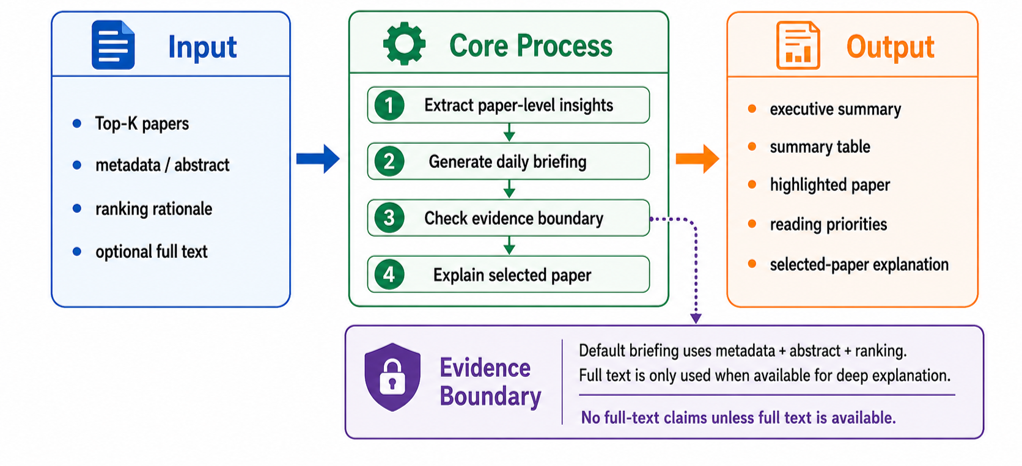
\includegraphics[width=0.9\linewidth]{skill2.png}
  \caption{ResearchSynthesisSkill consumes ranked recommendations and produces structured briefing items, daily briefing sections, and selected-paper explanations with visible evidence labels.}
  \label{fig:skill2-workflow}
\end{figure}

\section{Method}

The extraction stage converts ranking output into paper-level reading material. For each recommended paper, the Skill passes the title, abstract, score, rank, ranking rationale, and evidence source to the LLM provider. When the provider succeeds, the returned PaperBriefingItem contains paper-specific claims and reading guidance. When the provider fails, the Skill creates a deterministic fallback item from the available metadata and abstract, keeps the paper in the briefing, and exposes the fallback status through SkillResult.

The daily briefing stage organizes the extracted items into a user-facing report. It preserves the input ranking instead of reranking papers during synthesis. The summary table indexes Top-K papers, comparison notes explain differences among ranked items using allowed evidence, and reading priorities translate scores and claims into a practical reading order. Candidate-pool trend analysis is included only when enough candidates are available. The trend module counts repeated abstract terms, categories, and retrieval-source support, while downgrading query echoes that lack independent candidate evidence.

The selected-paper explanation stage supports deeper interaction after the daily briefing. Method mode focuses on the problem, method overview, workflow, inputs and outputs, and claimed innovation. Experiment mode covers datasets, baselines, metrics, setup, and conclusions. Limitations mode covers stated limitations, assumptions, missing validation, and risks. Source selection prioritizes user-provided full text, cached full text for the same PDF version, newly parsed PDF text, abstract-only fallback, and metadata-only fallback. When the Skill falls back to abstract or metadata, it labels missing experiment or limitation details instead of inventing them.

\section{Related Work}

The Skill follows the retrieval-augmented generation principle that generation should remain tied to retrieved evidence \citep{lewis2020}. It applies this principle at the Skill boundary: retrieval, ranking, and synthesis are separate stages, and each generated claim keeps a source label. Research on faithfulness in abstractive summarization shows that fluent summaries can contain unsupported content even when source documents are available \citep{maynez2020}. Hallucination surveys further motivate abstention and source-boundary reporting when evidence is incomplete \citep{ji2023}. In this project, default evidence consists of arXiv metadata and abstracts, while full-paper evidence is available only when PDF text is supplied or parsed \citep{arxivapi}.

\section{Results}

The evaluation is deterministic and fixture-backed. It uses fixed arXiv-like papers and a mock LLM provider, so the results are reproducible without live arXiv, live LLM calls, or PDF parsing. The briefing-quality evaluator checks required sections, Top-K coverage, trend status, reading priorities, evidence boundary, claim specificity, claim-support coverage, and forbidden full-text or PDF claims. Required-section coverage measures whether the briefing exposes all fields expected by the Agent. Top-K coverage measures whether every ranked paper appears in the summary table and paper-level briefing items. The explanation evaluator checks mode-specific field coverage. These metrics do not measure broad human preference, but they directly test whether the Skill satisfies the reportable contract required by the Agent.

\begin{table}[t]
  \centering
  \caption{ResearchSynthesisSkill fixture-backed evaluation.}
  \label{tab:skill2-results}
  \small
  \begin{tabular}{@{}lll@{}}
    \toprule
    Area & Metric & Result \\
    \midrule
    Daily briefing & Required enhanced sections & 1.000 \\
    Daily briefing & Top-K briefing coverage & 1.000 \\
    Daily briefing & Evidence boundary present & yes \\
    Daily briefing & Forbidden full-text or PDF claims & none \\
    Deep explanation & Method-mode completeness & 0.860 \\
    Fallback behavior & Missing or malformed evidence & structured result \\
    \bottomrule
  \end{tabular}
\end{table}

Table~\ref{tab:skill2-results} reports the main synthesis-side results used in the demo. The daily briefing reaches full required-section coverage and full Top-K coverage in the fixture setting. It also passes the evidence-boundary check because the default briefing marks full text as unused and avoids claims based on full-text evidence. The method-mode explanation reaches 0.860 completeness because the fixture intentionally omits one required method field. This result shows that the evaluator detects missing mode-specific information instead of accepting a polished but incomplete paragraph.

The qualitative demo further illustrates the output contract. Given ranked recommendations about arXiv research agents, the Skill produces a highlighted paper, comparison notes that distinguish ranking context from synthesis evidence, and reading priorities that map scores and claims to an ordered reading plan. When only abstracts are available, the evidence boundary explicitly marks full text as unavailable, so the final briefing remains useful without overstating the source material.

\section{Analysis}

The results show that the Skill can turn ranked rows into readable research decisions. This behavior depends on structured synthesis. A generic summary may be fluent, but it does not tell the user which paper to read first, which evidence supports a claim, or whether the system has access to the full paper. In contrast, this Skill exposes the summary table, per-paper items, comparison notes, reading priorities, and evidence boundary as separate fields. The user interface can render these fields directly, and tests can evaluate them without manual judgments about writing style.

\begin{table}[t]
  \centering
  \caption{Error-analysis behavior for evidence-limited synthesis.}
  \label{tab:skill2-errors}
  \small
  \begin{tabular}{@{}lll@{}}
    \toprule
    Condition & Controlled behavior & Effect \\
    \midrule
    Candidate pool absent & trend not assessed & avoids unsupported trend claims \\
    Too few candidates & insufficient data reported & preserves uncertainty \\
    Query echo only & signal downgraded & avoids circular evidence \\
    PDF parsing failure & abstract-only fallback & labels source limitation \\
    Missing method field & completeness below 1.0 & exposes incomplete evidence \\
    \bottomrule
  \end{tabular}
\end{table}

Table~\ref{tab:skill2-errors} explains why the evidence boundary is necessary. The Skill does not convert missing evidence into fluent but unsupported claims. Instead, it records not-assessed trend status, insufficient-data status, downgraded query echoes, abstract-only fallback, or incomplete explanation scores. These behaviors reduce the risk that the Agent confuses retrieval context, ranking context, and full-paper analysis.

\begin{thebibliography}{9}

\bibitem[arXiv(2026)]{arxivapi}
arXiv.
\newblock arXiv API User Manual.
\newblock \url{https://info.arxiv.org/help/api/user-manual.html}.

\bibitem[Ji et~al.(2023)]{ji2023}
Ziwei Ji, Nayeon Lee, Rita Frieske, Tiezheng Yu, Dan Su, Yan Xu, Etsuko Ishii, Ye Jin Bang, Andrea Madotto, and Pascale Fung.
\newblock Survey of hallucination in natural language generation.
\newblock ACM Computing Surveys, 55(12), Article 248, 2023.
\newblock \url{https://doi.org/10.1145/3571730}.

\bibitem[Lewis et~al.(2020)]{lewis2020}
Patrick Lewis, Ethan Perez, Aleksandra Piktus, Fabio Petroni, Vladimir Karpukhin, Naman Goyal, Heinrich Kuettler, Mike Lewis, Wen-tau Yih, Tim Rocktaschel, Sebastian Riedel, and Douwe Kiela.
\newblock Retrieval-augmented generation for knowledge-intensive NLP tasks.
\newblock Advances in Neural Information Processing Systems 33, pages 9459--9474, 2020.

\bibitem[Maynez et~al.(2020)]{maynez2020}
Joshua Maynez, Shashi Narayan, Bernd Bohnet, and Ryan McDonald.
\newblock On faithfulness and factuality in abstractive summarization.
\newblock Proceedings of the 58th Annual Meeting of the Association for Computational Linguistics, pages 1906--1919, 2020.
\newblock \url{https://doi.org/10.18653/v1/2020.acl-main.173}.

\end{thebibliography}

\end{document}
